Et båndpassfilter kan lages ved kaskadekobling av et LPF og et HPF.
Signalet legges ikke sammen, som ved en notch, men signalet fra det første
filteret mates inn i det neste.

\begin{figure}[H]
  \caption{båndpassfilter}
  \centering
  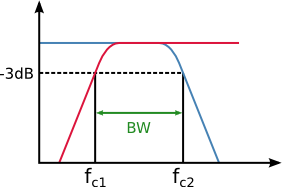
\includegraphics[width=0.5\textwidth]{./img/bp}
\end{figure}

$$BW = f_{c2} - f_{c1}$$
$$f_0 = \sqrt{f_{c1} \cdot f_{c2}}$$
$$Q = \frac{f_0}{BW}$$

\resizebox{\textwidth}{!}{
\begin{circuitikz} \draw
(6,5) node[op amp, yscale=-1] (opamp) {}
(opamp.+) node[left] {}
(opamp.-) node[left] {}
(opamp.out) node[right] {}

(-0.5,5.5) to[R, l=$R_2$] (1.5,5.5)
      to[R, l=$R_1$] (2.5,5.5)
      -- (opamp.+)
(3,5.5) to[C, l=$C_1$] (3,3.5)
      node[ground] {}

(1.25,5.5) -- (1.25,7)
      to[C, l=$C_2$] (7.5,7)
      -- (7.5,5)
(opamp.out) -- (8.5,5)

(opamp.-) -- (4.5,4.5)
      -- (4.5,3)
      -- (7.5,3)
      to[R, l=$R_{f1}$] (7.5,5)
(7.5,3) to[R, l=$R_{f2}$] (7.5,1)
      node[ground] {}



(14.5,4.5) node[op amp, yscale=-1] (opamp) {}
(opamp.+) node[left] {}
(opamp.-) node[left] {}
(opamp.out) node[right] {}

(8.5,5) to[C, l=$C_4$] (10.5,5)
      to[C, l=$C_3$] (11.5,5)
      -- (opamp.+)
(11.5,5) to[R, l=$R_3$] (11.5,3)
      node[ground] {}

(10.5,5) -- (10.5,6.5)
      to[R, l=$R_4$] (16,6.5)
      -- (16,4.5)
(opamp.out) -- (17.5,4.5)

(opamp.-) -- (13,4)
      -- (13,2.5)
      -- (16,2.5)
      to[R, l=$R_{f3}$] (16,4.5)
(16,2.5) to[R, l=$R_{f4}$] (16,0.5)
      node[ground] {}
      ;
\end{circuitikz}
} %resizebox
